\chapter{Esempi di sistemi dinamici continui}

\section{Alcuni sistemi meccanici}
\subsection{L'oscillatore armonico}
Considerimo l'equazione
\[\ddot x=-kx\]
con $k>0$ e $x\in \R$.\\
Studiamo il sistema equivalente
\[\begin{cases}
\dot x=y\\
\dot y=-kx
\end{cases}\]
con $(x,y)\in\R^2$ e $F(x,y)=(y,-kx)$.

\begin{itemize}
\item \textbf{Punti fissi}: $(y,-kx)=(0,0)\implies (x,y)=(0,0)$, quindi abbiamo un solo punto fisso.
\item Questo \`e evidentemente un sistema meccanico con $V(x)=\frac k2 x^2$, da cui $E(x,y)=\frac12 y^2+\frac k2 x^2$ \`e l'Hamiltoniana.
\item Sia $E_c=\cpa{\frac12y^2+\frac k2x^2=c}$. Questi insiemi sono evidentemente ellissi. Descrivono veramente orbite periodiche? S\`i, infatti se per assurdo non fossero orbite periodiche, poich\'e le orbite che cominciano in uno di questi insiemi sono costrette a rimanervi, per compattezza di $E_c$ dovremmo avere 
\[\ell=\lim_{t\to+\infty}\phi_t(x_0)\in E_c\] 
per $x_0\in E_c$, ma questo significa che $\ell$ sarebbe un punto fisso, che \`e assurdo perch\'e l'unico punto fisso \`e $(0,0)$.
\end{itemize}

\subsection{Pendolo semplice}
L'equazione in esame \`e
\[\ddot \theta=-\frac g\ell\sin\theta.\]
Riformuliamo in
\[\begin{cases}
\dot\theta=\psi\\
\dot\psi=-\frac g\ell\sin\theta
\end{cases}\]

\noindent
\textbf{Punti fissi}:\\
$\psi=0$ e $\sin\theta=0$, dunque
\[pt.fix=\cpa{(k\pi,0)\mid k\in\Z}.\]
\textbf{Integrale primo}:\\
Anche questo \`e un sistema meccanico, che quindi ammette Hamiltoniana
\[E(\theta,\dot\theta)=\frac12\dot\theta^2-\frac g\ell\cos\theta,\]
dunque gli insiemi di livello che ci interessano sono
\[E_c=\cpa{\frac12\psi^2-\frac g\ell\cos\theta=c}.\]
Osserviamo che
\[E(k\pi,0)=-\frac g\ell\cos(k\pi)=(-1)^{k+1}\frac g\ell\implies E(2\pi,0)=E(-2\pi)=E(0,0).\]
\[E_{-\frac{g}{\ell}}=\cpa{\frac12\psi^2-\frac g\ell\cos\theta=-\frac{g}{\ell}}\implies \psi^2=-2\frac g\ell(1-\cos\theta)\]
\[E_{\frac{g}{\ell}}=\cpa{\frac12\psi^2-\frac g\ell\cos\theta=\frac{g}{\ell}}\implies \psi^2=2\frac g\ell(1+\cos\theta)\]
Se $c\in\pa{-\frac g\ell,\frac g\ell}$ troviamo orbite periodiche contenute dentro le ondine dei primi due.\\
Per $c\notin \spa{-\frac g\ell,\frac g\ell}$ abbiamo invece ondine tutte sopra o tutte sotto.
\begin{figure}[!htb]
    \centering
    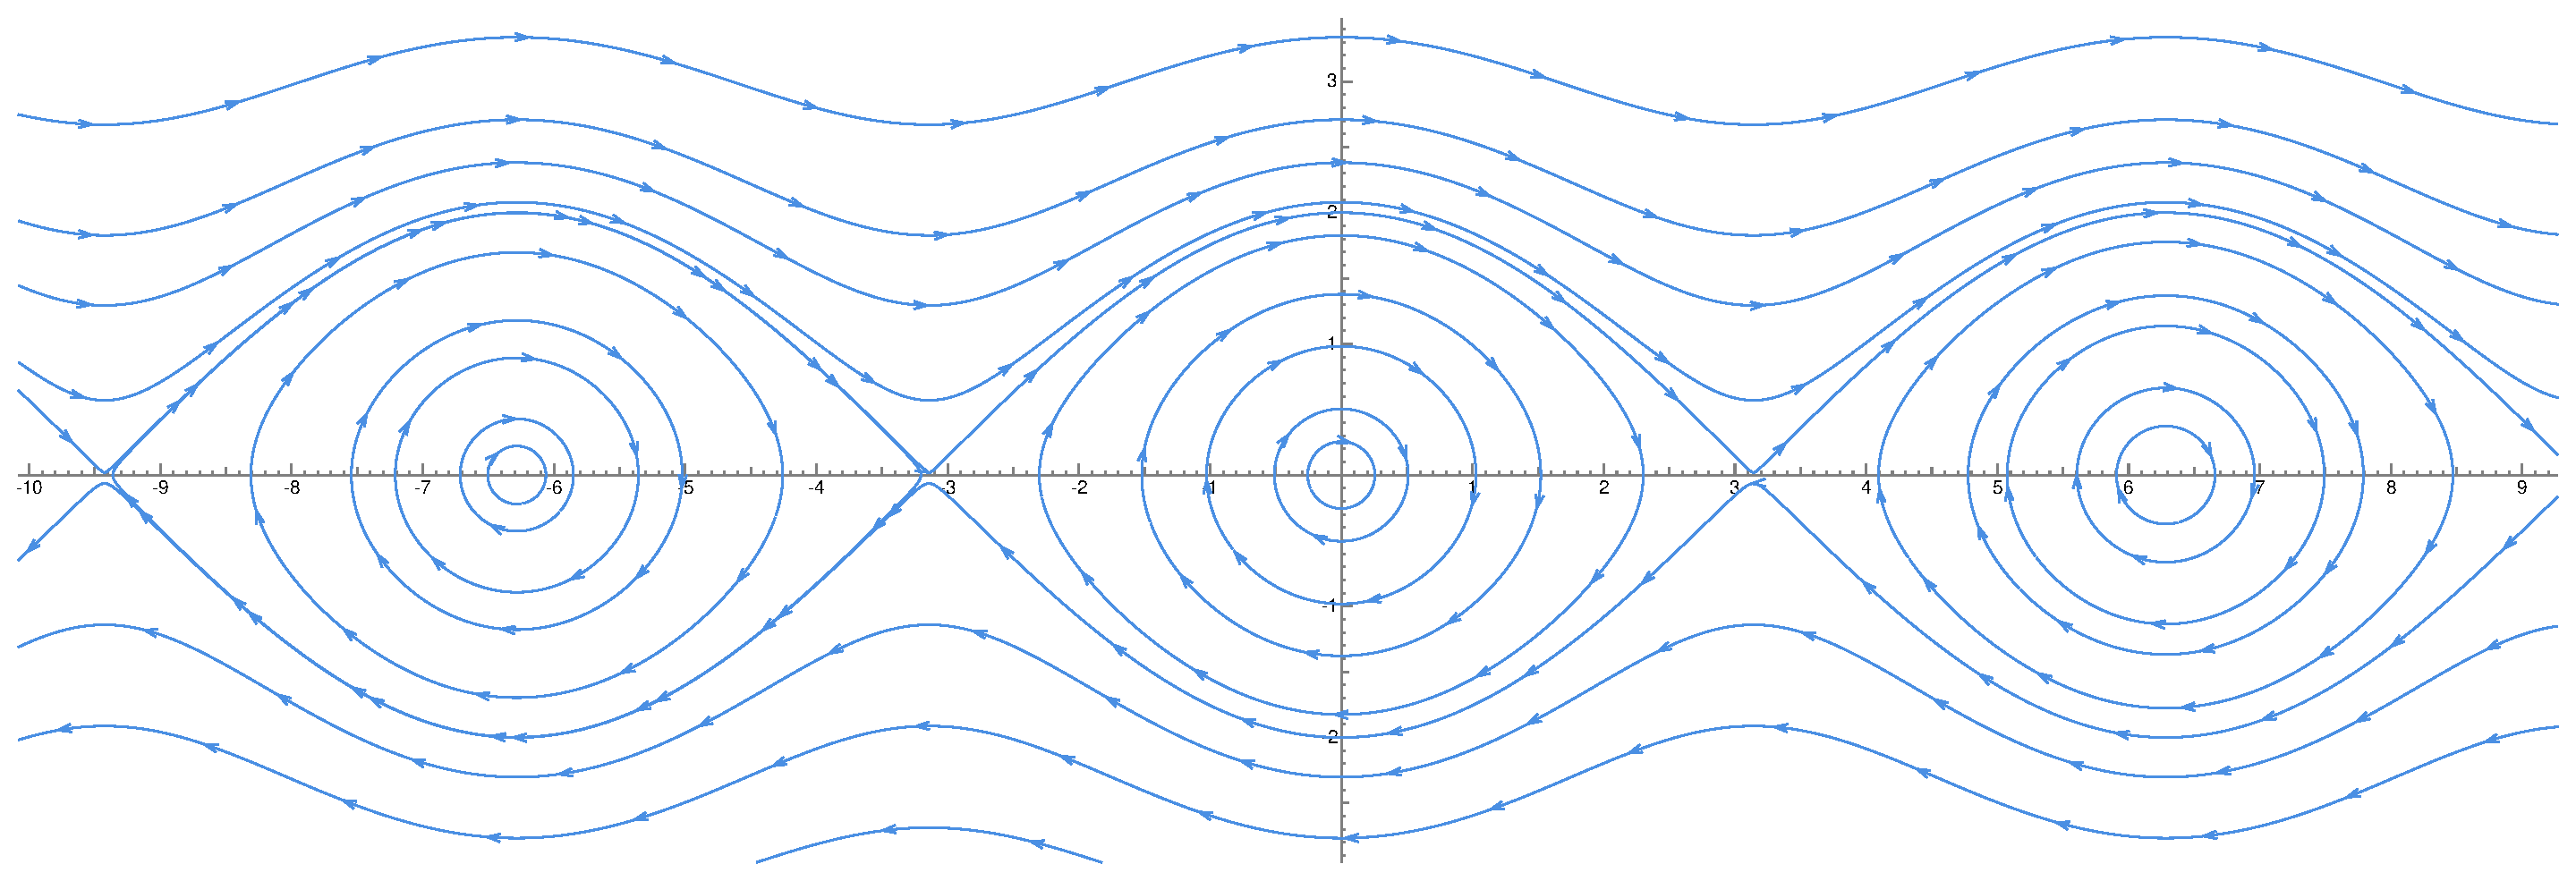
\includegraphics[width=11cm]{Immagini/pendolo.pdf}
    \caption{Diagramma di fase del pendolo per $\frac g\ell=1$}
\end{figure}



\section{Dinamica di Lotka-Volterra}
Possiamo modellare una singola popolazione in modo semplice con l'equazione (detta \textit{equazione logistica})
\[\dot x=x(c-a x),\quad a,c>0.\]
Ponendo $F(x)=xc-ax^2$ si ha che $F(x)=0\implies x=0$ oppure $x=c/a$.\\
Inserendo nel sistema una seconda popolazione che pi\`u interagire con la prima troviamo il sistema
\[\begin{cases}
\dot x=x(c_1-a_1x-b_1y)\\
\dot y=y(c_2-a_2y-b_2x)
\end{cases}.
\]
Osserviamo che gli assi sono invarianti. A meno di riscalamento possiamo considerare il sistema
\[\begin{cases}
\dot x=x(1-x-\al y)\\
\dot y=y(1-\beta x-y)
\end{cases}\]
Troviamo come punti fissi $(0,0)$, $(1,0)$, $(0,1)$ e
\[P=\pa{\frac{\al-1}{\al\beta-1},\frac{\beta-1}{\al\beta-1}}.\]
Osserviamo che $P\in\cpa{x>0,y>0}$ se e solo se $\al>1$ e $\beta>1$ o $0<\al<1$ e $0<\beta<1$.\\
Calcoliamo ora $\Dc F$
\[\Dc F=\mat{1-2x-\al y & -\al x\\ -\beta y & 1-\beta x-2y}.\]
Segue che
\begin{gather*}
\Dc F((0,0))=\mat{1 & 0\\ 0 & 1},\\
\Dc F((1,0))=\mat{-1 & -\al\\ 0 &1-\beta},\quad
\Dc F((0,1))=\mat{1-\al & 0\\ -\beta & -1},\\
\Dc F(P)=\frac 1{\al \beta -1}\mat{
    1-\al &
    \al(1-\al)\\
    \beta(1-\beta) &
    1-\beta
}.
\end{gather*}

\begin{example}
Consideriamo il modello Lotka-Volterra dato da $\al=2$ e $\beta=2$, cio\`e
\[\begin{cases}
\dot x=x(1-x-2y)\\
\dot y=y(1-2x-y)
\end{cases}\]
Per quanto detto sopra i punti fissi sono
\[(0,0),\ (1,0),\ (0,1),\ \pa{\frac13,\frac13},\]
che nominiamo rispettivamente $P_0,\ P_1,\ P_2$ e $P_3$.\\
Segue che $P_0$ \`e una stella instabile, $P_1$ e $P_2$ sono nodi impropri stabili e $P_3$ \`e una sella.
Gli autovettori di $\Dc F(P_3)=-\frac13\pa{\smat{1 &2\\2&1}}$ sono $v_+=(1\ -1)^\top$ e $v_-=(1\ 1)^\top$, corrispondenti agli autovalori $1/3$ e $-1$ rispettivamente. Graficando il sistema possiamo effettivamente notare che le variet\`a instabili e stabili hanno come giacitura della retta tangente in $P_3$ proprio le rette generate da questi vettori.
\begin{figure}[!htb]
    \centering
    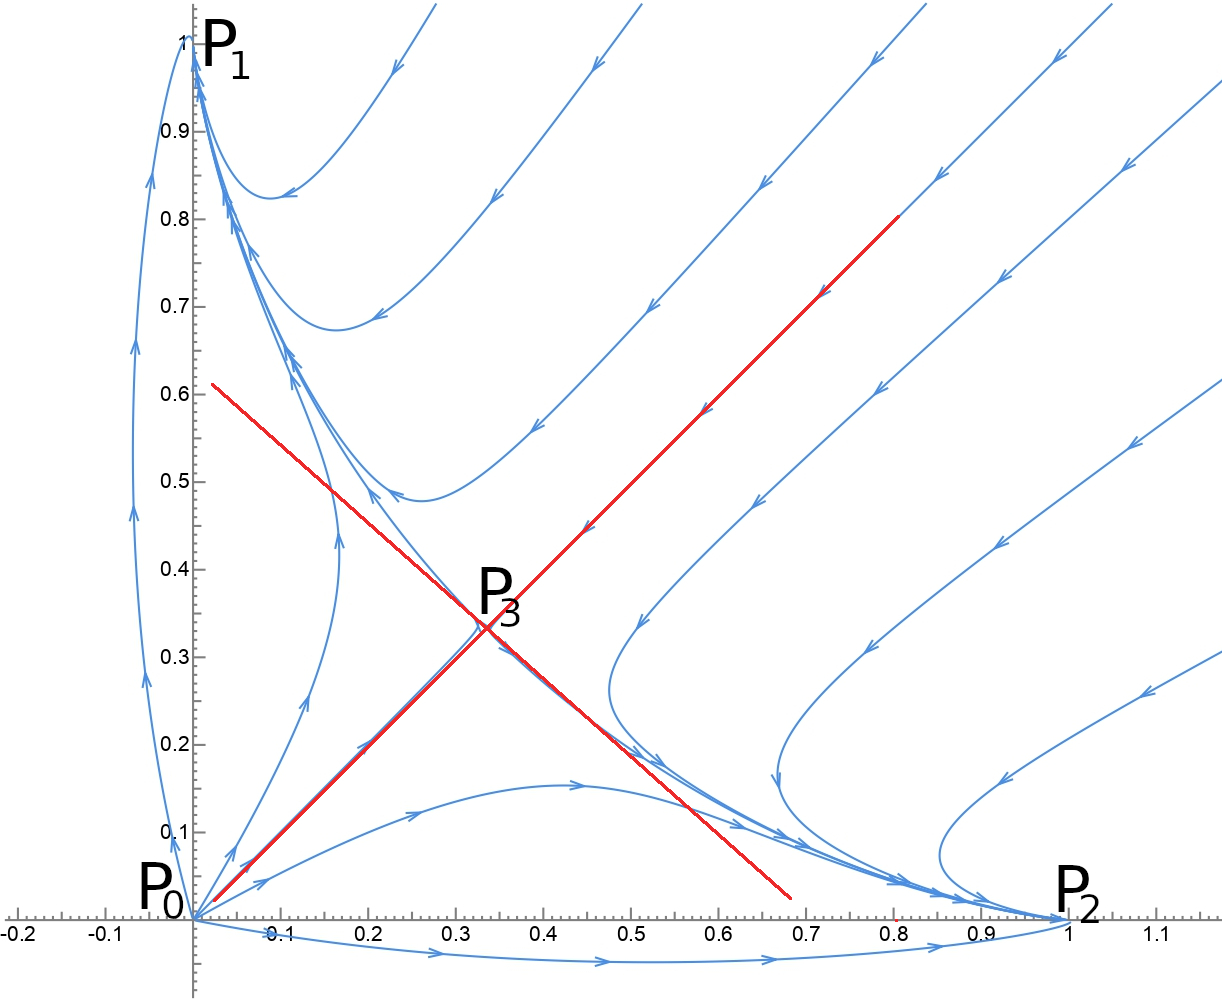
\includegraphics[width=8cm]{Immagini/Lotka-VolterraVarietaStabili.jpg}
    \caption{Diagramma di fase di questo sistema.\\
    In rosso sono indicati $P_3+\Span(v_+)$ e $P_3+\Span(v_-)$.}
\end{figure}

\end{example}

\begin{example}[Lotka-Volterra per preda-predatore]
Consideriamo il sistema
\[\begin{cases}
\dot x= x(-1+y)\\
\dot y=y(1-x)
\end{cases}\]
I punti fissi sono $(0,0)$ e $(1,1)$. Osserviamo anche che gli assi e tutto il primo quadrante sono insiemi invarianti. Consideriamo allora solo il primo quadrante che tanto \`e il caso interessante per questo modello.\\
Studiamo lo Jacobiano
\[\Dc F(x,y)=\mat{-1+y & x\\ -y & 1-x}\implies \Dc F(0,0)=\mat{-1 &0\\0&1},\ \Dc F(1,1)=\mat{0 & 1\\ -1 &0}.\]
\setlength{\leftmargini}{0cm}
\begin{itemize}
\item[$\boxed{(0,0)}$] $(0,0)$ \`e una sella. Si ha che 
\[E^s(0,0)=\Span\mat{1\\0}\quad E^u(0,0)=\Span\mat{0\\ 1}\]
e per il teorema delle variet\`a stabili locali (\ref{TeoremaVarietaStabileInstabile}) sappiamo che $W^s(0,0)$ e $W^u(0,0)$ locali esistono e sono uniche. Per l'invarianza degli assi in realt\`a $W^{u/s}(0,0)=E^{u/s}(0,0)$.
\item[$\boxed{(1,1)}$] $(1,1)$ \`e di tipo centro e quindi non \`e iperbolico. Una possibile funzione di Lyapunov potrebbe avere forma 
\[V(x,y)=a(x-1)^{2n}+b(y-1)^{2m},\quad a,b>0,\ n,m\in \N.\]
Un altro metodo potrebbe essere studiare il punto passando a coordinate polari centrate in $(1,1)$.\\
Un'ulteriore possibilit\`a potrebbe essere studiare il segno del campo di vettori, ma poich\'e $(1,1)$ \`e di tipo centro non \`e molto utile.\\
Trovare insiemi invarianti non \`e molto facile in questo caso.\\
Possiamo provare il metodo delle isocline
\[\begin{cases}
\dd yx=\frac{y(1-x)}{x(-1+y)}\\
y(x_0)=y_0\ t.c. x_0(-1+y_0)
\end{cases}\]
\`E chiaro che possiamo trarre qualche beneficio dal metodo delle isocline perch\'e l'equazione differenziale in questione \`e separabile
\[\frac{-1+y}ydy=\frac{1-x}xdx\implies \int_{y_0}^{y(x)}\frac{-1+y}ydy=\int_{x_0}^{x}\frac{1-x}xdx\]
\[y(x)-\log(y(x))=\log y_0-y_0+\log x-x-\log x_0+x_0.\]
Non posso scrivere esplicitamente $y(x)=$``qualcosa", ma comunque posso studiare l'equazione, infatti, poich\'e $\cpa{y=y(x)}$ \`e invariante (\ref{MetodoIsoclineNelPiano}) sappiamo che c'\`e un insieme invariante. Per identificarlo definiamo
\[I(x,y)=y-\log y+x-\log x.\]
Segue che\footnote{pensando $c=\log y_0-y_0-\log x_0+x_0$}
\[\dot I\res{I=c}=\pa{1-\frac1x}x(-1+y)+\pa{1-\frac1y}y(1-x)=0,\]
cio\`e $I$ \`e un integrale primo.
\[\nabla I(1,1)=\mat{1-\frac1x\\1-\frac1y}\res{(x,y)=(1,1)}=\mat{0\\0}.\]
\[H_I(x,y)=\mat{\frac1{x^2}&0\\ 0&\frac1{y^2}}\res{(x,y)=(1,1)}=\mat{1&0\\0&1}\implies\text{minimo locale}.\]
Troviamo dunque che localmente le traiettorie sono curve semplici chiuse tali che $(1,1)$ si trova nella componente connessa limitata tra le due che hanno come bordo le traiettorie.\\
Per trovare il verso di percorrenza possiamo usare il segno del campo.
\end{itemize}
\setlength{\leftmargini}{0.5cm}
\end{example}


\begin{example}
Un esempio semplice per i parametri del modello sopra \`e
\[\begin{cases}
\dot x=x(3-x-2y)\\
\dot y=y(2-y-x)
\end{cases}\implies F(x,y)=(x(3-x-2y),y(2-x-y)).\]

\begin{figure}[!htb]
    \centering
    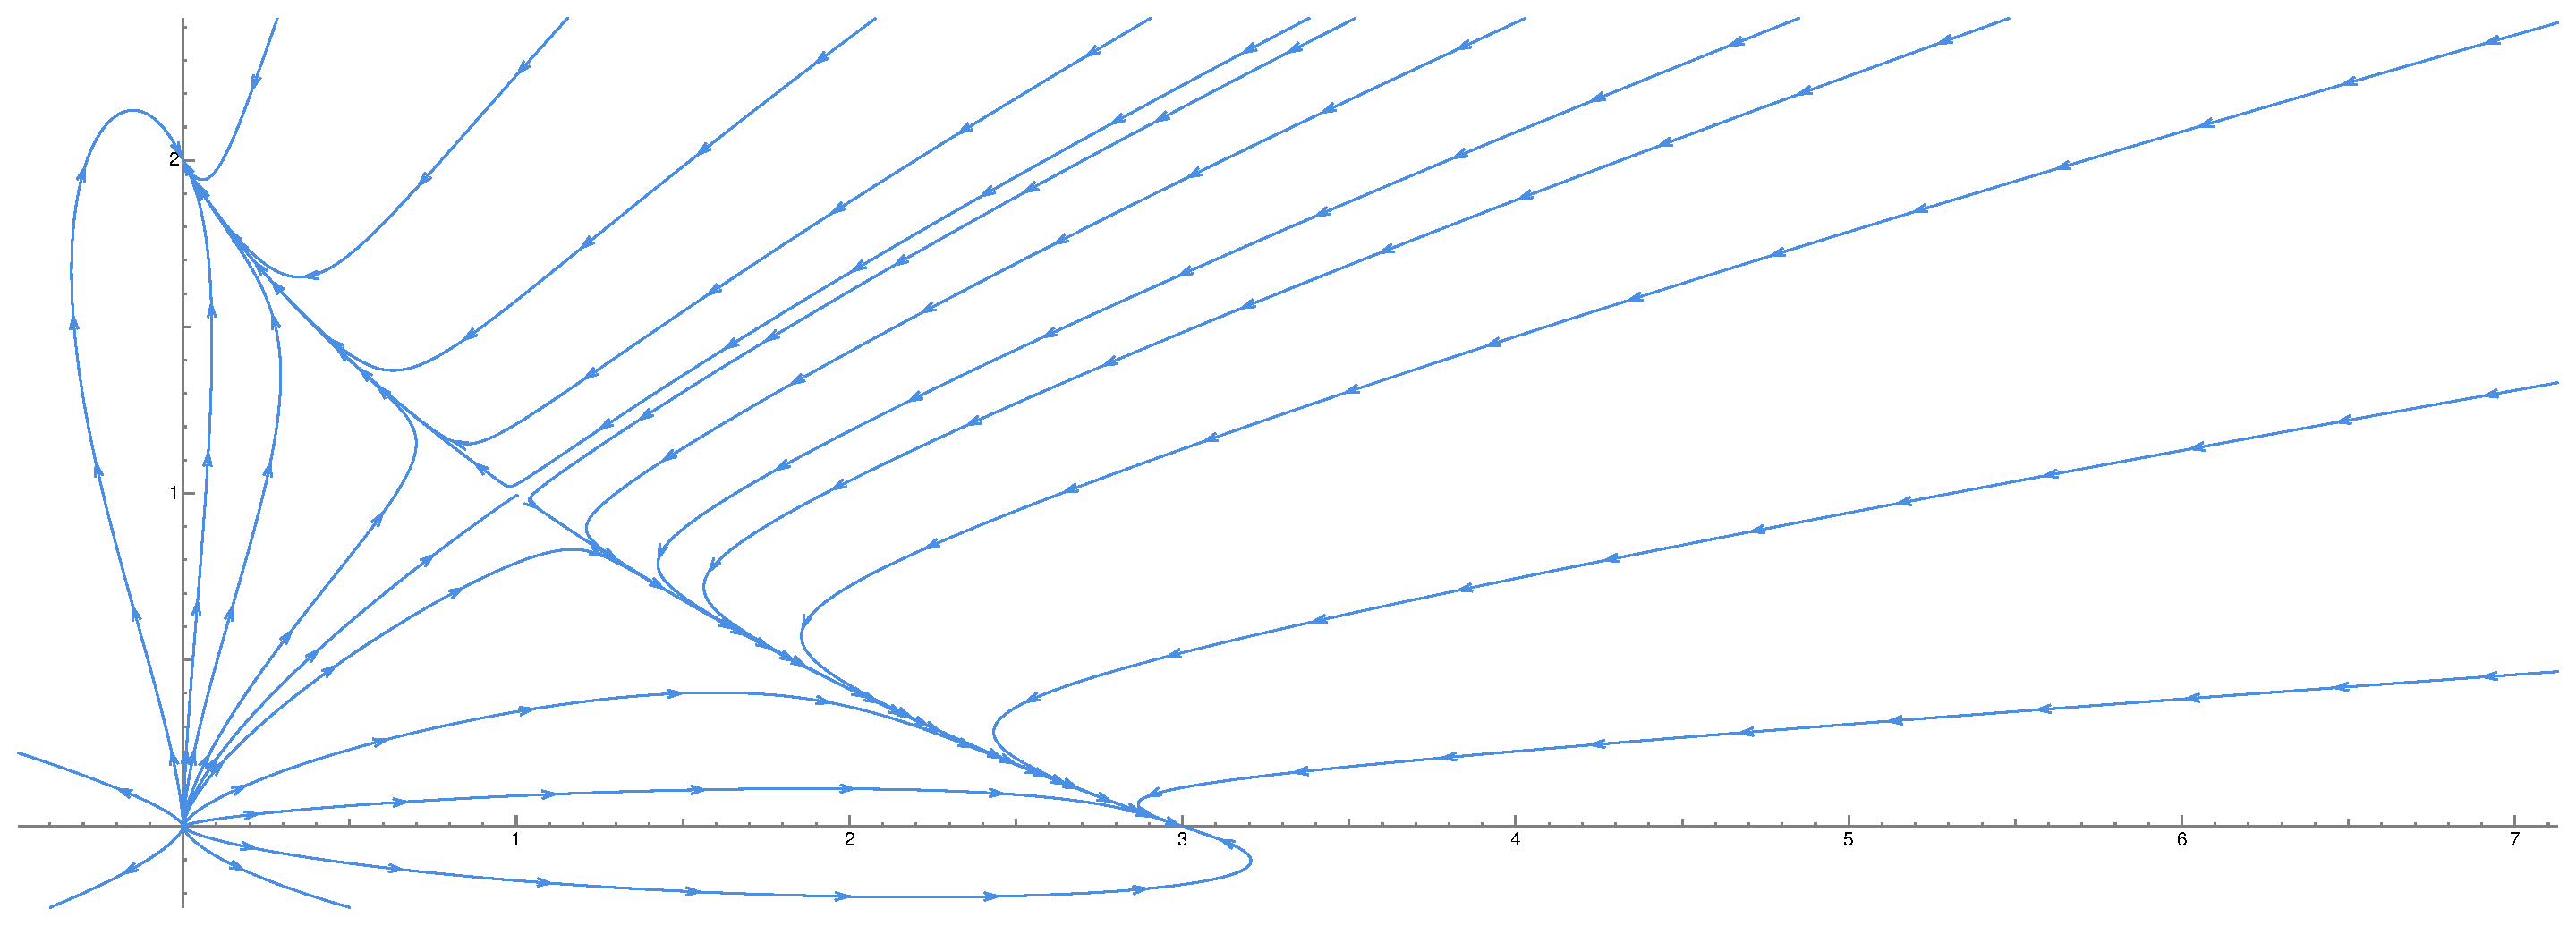
\includegraphics[width=11cm]{Immagini/LotkaVolterra.pdf}
    \caption{Diagramma di fase per questo esempio di Lotka-Volterra.}
\end{figure}

\noindent
I punti fissi sono
\[(0,0),\ (0,2),\ (3,0),\ (1,1)\]
e la matrice Jacobiana di $F$ \`e
\[\Dc F(x,y)=\mat{3-2x-2y & -2x\\
-y & 2-x-2y}.\]
Valutando lo Jacobiano nei punti fissi troviamo
\[\under{\text{nodo instabile}}{\mat{3 & 0\\0&2}},\ \under{\text{nodo stabile}}{\mat{-1 &0\\ -2 &-2}},\ \under{\text{nodo stabile}}{\mat{-3 &-6\\0 &-1}}, \under{\text{sella}}{\mat{-1 & -2\\ -1 & -1}}.\]
\end{example}


\section{Sistema di Lorenz}
Un sistema storicamente importante \`e il seguente:
\[\begin{cases}
\dot x = \sigma(-x+y)\\
\dot y = rx-y-xz\\
\dot z = -bz+xy
\end{cases},\quad r,b,\sigma\in\R^+.\]
Osserviamo che i punti fissi del sistema corrispondono a
\[P_0=\mat{0\\0\\0},\quad P_+=\mat{\sqrt{b(r-1)}\\\sqrt{b(r-1)}\\r-1},\quad P_-=\mat{-\sqrt{b(r-1)}\\-\sqrt{b(r-1)}\\r-1},\]
dove $P_\pm$ \`e definito solo per $r\geq1$. Osserviamo inoltre che
\[\Dc F=\mat{-\sigma&\sigma&0\\r-z&-1&-x\\y&x&-b}.\]
Studiamo la stabilit\`a di $P_0$:\\
Notiamo che
\[\Dc F(P_0)=\mat{-\sigma&\sigma&0\\
r&-1&0\\0&0&-b},\]
dunque $(0,0,1)$ \`e sempre un autovettore relativo all'autovalore $-b$ per il sistema linearizzato vicino a $P_0$. Il segno di $-b$ ci dice che $\dim E^s(P_0)\geq1$. Studiamo la stabilit\`a delle altre direzioni al variare di $r$ 
\setlength{\leftmargini}{0cm}
\begin{itemize}
\item[$\boxed{r\in(0,1)}$] In questo caso gli autovaori sono entrambi con parte reale negativa, quindi per Hartman Grobman (\ref{TeoremaHartmanGrobman}) $P_0$ \`e asintoticamente stabile e $\dim E^s(P_0)=3$.
\item[$\boxed{r>1}$] In questo caso gli autovalori sono reali di segno opposto dunque il punto fisso \`e instabile per Hartman Grobman (\ref{TeoremaHartmanGrobman}) e $\dim E^s(P_0)=2,\ \dim E^u(P_0)=1$.
\item[$\boxed{r=1}$] In questo caso $P_0$ non \`e iperbolico dunque per predicare sulla stabilit\`a proviamo a cercare una funzione di Lyapunov. Tentiamo una di questa forma
\[V(x,y,z)=\frac12(k_1x^2+k_2y^2+k_3z^2).\]
Chiaramente $V$ \`e di classe $C^1$ e $V(P)>V(P_0)=0$ per ogni $P\in\R^3\bs\cpa{P_0}$. Cerchiamo delle condizioni sui $k_i$ in modo tale che $\dot V(P)\leq 0$ per ogni $P\neq P_0$. Dopo qualche conto si pu\`o verificare che
\[V(x,y,z)=\frac12\pa{\frac1\sigma x^2+y^2+z^2}\]
\`e una funzione di Lyapunov (non stretta). Per il primo teorema di Lyapunov (\ref{TeoremaLyapunov1Stabilita}) segue che $P_0$ \`e stabile.\\
Per il criterio di La Salle (\ref{CriterioLaSalle}) sappiamo che $\cpa{\dot V=0}=\cpa{x=y,z=0}$ contiene tutti gli $\omega$-limiti e che questi sono insiemi invarianti. Poich\'e
\[F\res{\cpa{x=y,z=0}}=\mat{0\\0\\x^2}\]
si ha che $\cpa{P_0}$ \`e l'unico insieme invariante contenuto in $\cpa{\dot V=0}$, dunque tutti gli $\omega$-limiti sono $\cpa{P_0}$. Questa condizione insieme alla stabilit\`a di $P_0$ mostra che $P_0$ \`e asintoticamente stabile.
\end{itemize}
\setlength{\leftmargini}{0.5cm}
Attraverso conti non visti a lezione sappiamo che se $\sigma>b+1$ e $r>\ol r$ per un qualche $\ol r>1$ si ha che $\dim E^s(P\pm)=1$ e $\dim E^u(P_\pm)=2$. Le traiettorie dunque approcciano $P_+$ e $P_-$ ``lateralmente" e ``trasversalmente" si allontanano lungo una spirale.

Sempre attraverso conti non visti a lezione individuiamo la funzione
\[W(x,y,z)=\frac12(rx^2+\sigma y^2+\sigma(z-2r)^2),\]
il cui dot \`e dato da
\[\dot W(x,y,z)=-\sigma(rx^2+y^2+b(z-r)^2-br^2).\]
Osserviamo che, fissato $k\in\R^+$ possiamo trovare $c\in\R$ tale che $\dot W\res{W\geq c}\leq -\sigma k<0$: basta prendere $c$ grande abbastanza in modo tale che i punti fuori l'ellissoide $\cpa{W=c}$ abbiano coordinate grandi abbastanza da forzare la disuguaglianza voluta, che possiamo fare per il segno dei termini in $\dot W$.\\
Osserviamo che se $y_0\notin \cpa{W\geq c}$ allora
\[W(\phi_t(y_0))-W(y_0)=\int_0^t\under{=\dot W}{\dd s{}W(\phi_s(y_0))}ds\leq -k\sigma t\]
finch\'e $\phi_t(y_0)$ continua ad essere fuori l'ellissoide. Segue dunque che definitivamente $\phi_t(y_0)$ cade nell'ellissoide.

Questo ragionamento mostra che tutti i punti ammettono $\omega$-limite, ma questo non pu\`o in generale essere un punto fisso (sono instabili) o un'orbita periodica (perch\'e assenti dal sistema\footnote{questa affermazione non \`e stata mostrata}). Si scopre che l'$\omega$-limite generale corrisponde ad un frattale e per questo motivo viene detto \textit{attrattore strano}.

\begin{figure}[!htb]
    \centering
    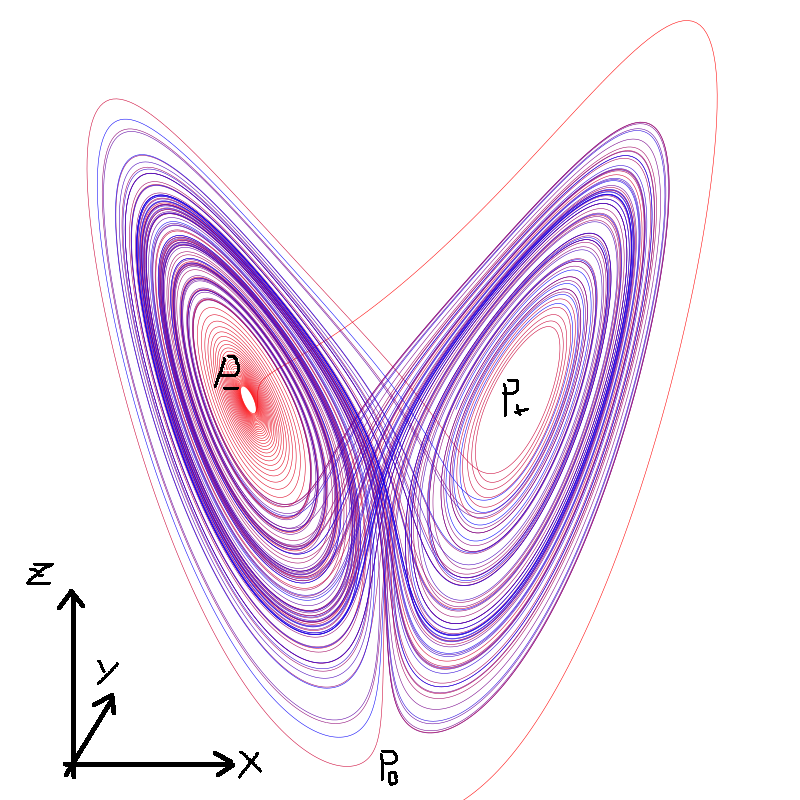
\includegraphics[width=8cm]{Immagini/800px-Lorenz_attractor.png}
    \caption{Qualche orbita del sistema di Lorenz dove sono stati contrassegnati i punti fissi. Immagine originariamente da \url{https://en.wikipedia.org/wiki/Lorenz_system} e modificata da me.}
\end{figure}




